\chapter{Metamodelling} \label{metamodelchapter}

\section{Introduction} \label{metamodelintro}

\section{Defining a Modelling Language} \label{languagedef}

\subsection{Components of a Modelling Language} \label{langcomponents}

%-Modeling Language Requirements and Features
%===========================================
%defining modeling languages comes in section \ref{languagedef}
%no single set of constructs and features that will satisfy all needs -> profiles
%static language used to represent collections of structured data; dynamic language is used to represent executable actions (Tony's `Defining Languages in XMT')
%large scale reuse (templates?) - consistent architecture (for enterprise/system models, business models, metamodels (a.s, c.s., semantics) -> templates can help \cite{mdadsouza}
%constraint language

%make distinction from `features' of a modeling language
%James formal semantics of programming book

%\subsection{Modeling vs. Programming Languages}
%\subsection{Principles of Modeling Language Design}
%\subsection{Formal vs. Informal Semantics} \label{formalintro}
%\subsection{Approaches to Formalising Semantics}
%\subsection{Formal vs. Metamodeling Languages}

\section{Metamodel Architecture} \label{metamodelarch}

\subsection{MOF and the Four-Layer Architecture} \label{mof}

%MDA is not a single technology itself, but a unifying framework for a number of related model-driven technologies and standards, such as UML, the Meta-Object Facility (MOF) and XMI.

%UML has become the \textit{de facto} modeling language since its adoption in 1997, and is used for modeling all aspects of software systems throughout the development lifecycle (the system modeling space). UML is described in more detail in section \ref{mdsdlang}.

%Whilst there are number of ways of defining languages such as UML (see section \ref{languagedef}), in MDA language specifications are themselves models (known as \emph{metamodels}), which are defined as instances of the Meta Object Facility. MOF is a language for specifying technology neutral metamodels and for implementing repositories of metadata \cite{mofspec}. The syntaxes of MOF and UML are quite similar, but because of their different usage scenarios (MOF is used primarily for defining languages, UML for describing systems), they are not totally aligned \cite{mofspec}. The OMG specifies an architecture for relating the various system models and language metamodels, which is depicted in Figure \ref{figmetamodelarch}. The relationship between models at consecutive levels is one of instantiation. Note that the specification for MOF is defined as an instance of itself to eliminate the need for a layer above M3. MOF and the metamodel architecture (particularly the limitations of the four layer architecture) are discussed in detail in section \ref{metamodeling}.

%\begin{figure}[htb]
%\begin{center}
%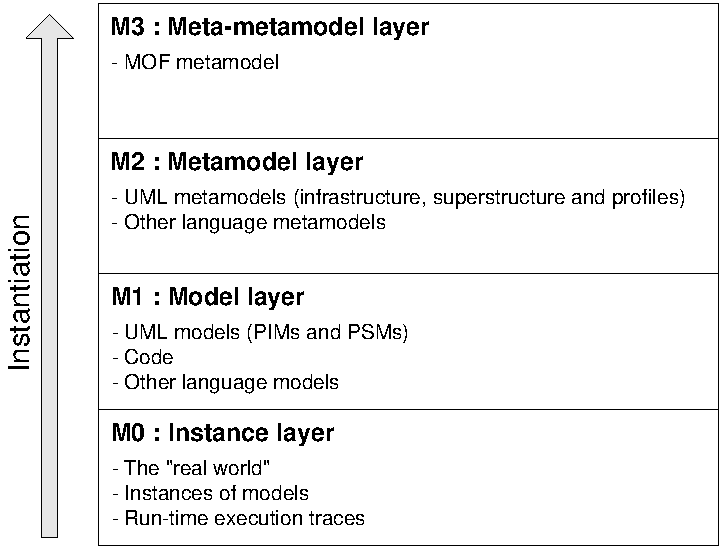
\includegraphics[width=8cm]{ModelDrivenDevelopment/figures/metamodelarch.pdf}
%\caption{\textbf{The OMG Four Layer Metamodel Architecture.}}
%\label{figmetamodelarch}
%\end{center}
%\end{figure}

%Another important aspect of MDA is that models should be freely interchangeable between tools and repositories, as highlighted in section \ref{mdavision}. In order to enable this, OMG has adopted an interchange standard called the XML Metadata Interchange (XMI) \cite{xmispec}. XML is a syntax for representing structural data in a textual form. The valid structure of a particular set of XML documents can be captured in an XML DTD (Document Type Definition) or schema - any XML document can be then be checked against the appropriate DTD or schema for well-formedness. XMI allows MOF metamodels and UML models to be represented as XML documents. These be checked against the MOF DTD or UML DTD respectively for well-formedness. Because languages other than UML can be defined using MOF, XMI also provides a facility for generating an appropriate DTD for any MOF compliant metamodel, so the well-formedness of instances of that metamodel can be checked.

\subsection{A Reflective Metamodel Architecture} \label{reflection}

\section{Architecture of a Language Metamodel} \label{langarchitecture}

\section{Process for Constructing Language Metamodels} \label{metamodellingprocess}

%need abstract syntax, semantics and interpreter, and THAT's IT!
%reflection?


% LITERATURE REVIEW
%==================

%\section{Metamodeling} \label{metamodeling}

%\subsection{Metadata and Metamodels} \label{metadata}

%data about data - equivalent to models
%MDR - metadata repository
%MOF
%code as model - code does not need to be a UML model but it must be an instance of a MOF metamodel
%data warehousing / CWM
%tools understanding metamodeling language -> customisable; guis as models (see tools above)
%syntax, semantics, constraints, concrete syntax

%Metatools
%=========
%tools understanding metamodeling language -> customisable; guis as models
%mdsd - tools (gui) etc. as models; move away from bespoke
%metatools: MetaEdit+, Dome, PROGRESS (graph grammars), MMT \cite{pumlmda}, KMF, XMT, IBM EMF (EMF.Edit, EMF.Codegen)
%tools should be able to export instances of their models in XMI that is a valid instance of a metamodel (e.g. UML metamodel) (*ANDYBAE*)
%tools should be able to supply info about their metamodel in a form that is a valid instance of an appropriate meta-metamodel (e.g. MOF) (*ANDYBAE*)


%\subsection{Requirements for a Metamodeling Language}

%\subsection{Architectures for Metamodeling} \label{metaarch}

%supposed advantages of fixed metamodel architecture (\cite{mofspec} p.2-3)

%\subsection{Fixed vs. Reflective Architectures}

%\subsection{Architectural Problems} \label{archprobs}

%already outlined in \ref{introarchfix}!
%Instantiation and Meta-instantiation
%problems with kuhne work!
%consistent architecture (for enterprise/system models, business models, metamodels (a.s, c.s., semantics) \ref{mdsdarch}
%nature of metamodel architecture : fixed vs. reflexive, translational vs. extensional approach to semantics; where do semantics live, where do mappings live; how to map different views of UML? what about inter-layer mappings? what about the definition of the architecture itself?
%translational vs. extensional approach? (MOF vs. infrastructure vs. superstructure): "as far as possible, new constructs should be defined by translation to the core, rather than have independently defined semantics" \cite{mdadsouza}
%translation - good: all superstructure maps down onto a simpler domain, and mapping is all at abstract syntax level; bad: information in original model can potentially be lost (Andy e-mail "Re: Superstructure vs. Infrastructure", 19 March 2002)
%models have been used in the software development process for some time, but the resultant models are intermediate artefacts leading to code, rather than valuable artefacts in themselves; failure to unite different views; need to separate meaning from representation;``each of UML's myriad diagrams is then merely a projection of the underlying language specification'' \cite{mellor}


%\subsection{Languages for Metamodeling}

%XMI not rich enough

%\subsection{The OMG's Meta-Object Facility}
%limitations of MOF
%MOF too repository biased. Should be able to model check etc.
%why O-O? (see \ref{oo}). Not just for modeling OO software 